\documentclass[../Report.tex]{subfiles}

\begin{document}


\chapter{Test}
\label{chap:test}
Der erste Plot test
\begin{figure}[h!]
	\centering
	\newlength\figureheight
	\newlength\figurewidth
	\setlength\figureheight{10cm}
	\setlength\figurewidth{15cm}
	% This file was created by matplotlib2tikz v0.6.17.
\begin{tikzpicture}

\definecolor{color0}{rgb}{0.12156862745098,0.466666666666667,0.705882352941177}

\begin{axis}[
xlabel={t in \si{\second}},
ylabel={U in \si{\milli \volt}},
xmin=-5.55555555555e-08, xmax=1.1666666666655e-06,
ymin=-150.03620886285, ymax=173.07157201985,
width=\figurewidth,
height=\figureheight,
tick align=outside,
tick pos=left,
x grid style={white!69.01960784313725!black},
y grid style={white!69.01960784313725!black},
legend cell align={left},
legend entries={{$U_?(t)$}},
legend style={draw=white!80.0!black}
]
\addlegendimage{no markers, color0}
\addplot [semithick, color0]
table {%
0 0.0631801395115
5.05050505051e-09 -1.77989959787
1.0101010101e-08 -4.97683128447
1.51515151515e-08 0.758228429418
2.0202020202e-08 -0.0233760248143
2.52525252525e-08 -5.55976528992
3.0303030303e-08 1.10411011548
3.53535353535e-08 -1.47695898918
4.0404040404e-08 -4.65656354398
4.54545454545e-08 0.483512572169
5.05050505051e-08 -2.30875543129
5.55555555556e-08 -3.42629548084
6.06060606061e-08 -0.875401068109
6.56565656566e-08 0.0108396384719
7.07070707071e-08 -3.43309823805
7.57575757576e-08 -3.33758012721
8.08080808081e-08 1.12637963503
8.58585858586e-08 -4.08623969461
9.09090909091e-08 -2.20736307945
9.59595959596e-08 1.30467769326
1.0101010101e-07 -4.88659051438
1.06060606061e-07 -2.36623564498
1.11111111111e-07 -0.111526987384
1.16161616162e-07 -2.07428925137
1.21212121212e-07 -3.10151893976
1.26262626263e-07 -1.81436314207
1.31313131313e-07 -0.476538651539
1.36363636364e-07 -4.62325962688
1.41414141414e-07 -0.272716699299
1.46464646465e-07 -0.64101292298
1.51515151515e-07 -6.226451084
1.56565656566e-07 0.378230654488
1.61616161616e-07 -0.687564330841
1.66666666667e-07 -3.16995456436
1.71717171717e-07 -1.57078872355
1.76767676768e-07 -2.2105193105
1.81818181818e-07 -0.782929081023
1.86868686869e-07 -2.9365139872
1.91919191919e-07 0.15205402013
1.9696969697e-07 -1.5476879068
2.0202020202e-07 -5.0409902468
2.07070707071e-07 1.39084536903
2.12121212121e-07 -2.24725790909
2.17171717172e-07 -2.56292812117
2.22222222222e-07 -0.698031413078
2.27272727273e-07 -3.46161934428
2.32323232323e-07 -0.475785169613
2.37373737374e-07 -3.01900354958
2.42424242424e-07 -0.916155125589
2.47474747475e-07 -1.85619922775
2.52525252525e-07 -4.82553277179
2.57575757576e-07 1.04005762231
2.62626262626e-07 -4.59553170805
2.67676767677e-07 -3.25551243262
2.72727272727e-07 0.0526884327404
2.77777777778e-07 -4.37426508287
2.82828282828e-07 -1.40389832508
2.87878787879e-07 -3.36657036358
2.92929292929e-07 -0.516424687969
2.9797979798e-07 -2.58273433374
3.0303030303e-07 -4.0800799656
3.08080808081e-07 2.91232598081
3.13131313131e-07 -6.58730020479
3.18181818182e-07 -0.805033216846
3.23232323232e-07 1.54746571685
3.28282828283e-07 -6.60022614277
3.33333333333e-07 3.33250022539
3.38383838384e-07 -5.93878793758
3.43434343434e-07 0.863001502512
3.48484848485e-07 3.28154211911
3.53535353535e-07 -20.9892606587
3.58585858586e-07 33.7386125095
3.63636363636e-07 103.532197312
3.68686868687e-07 97.0215309354
3.73737373737e-07 88.0224345888
3.78787878788e-07 118.998978278
3.83838383838e-07 147.261140584
3.88888888889e-07 143.009431907
3.93939393939e-07 147.924690797
3.9898989899e-07 150.503725729
4.0404040404e-07 141.33444138
4.09090909091e-07 158.384854707
4.14141414141e-07 145.791318154
4.19191919192e-07 116.995509957
4.24242424242e-07 118.970459313
4.29292929293e-07 104.374834889
4.34343434343e-07 78.1281255014
4.39393939394e-07 57.4405797416
4.44444444444e-07 28.1596219042
4.49494949495e-07 -11.7209630108
4.54545454545e-07 -31.8265901255
4.59595959596e-07 -36.885259047
4.64646464646e-07 -74.2941293526
4.69696969697e-07 -95.199383659
4.74747474747e-07 -95.998333098
4.79797979798e-07 -118.664634193
4.84848484848e-07 -129.363878229
4.89898989899e-07 -135.137944973
4.94949494949e-07 -135.34949155
5e-07 -135.297959786
5.05050505051e-07 -134.949287501
5.10101010101e-07 -118.824089647
5.15151515152e-07 -119.281798375
5.20202020202e-07 -93.6830909742
5.25252525253e-07 -72.5291882726
5.30303030303e-07 -75.3949985907
5.35353535354e-07 -26.9873547307
5.40404040404e-07 -24.2443994151
5.45454545455e-07 -6.37597691825
5.50505050505e-07 86.3157452089
5.55555555556e-07 36.9473808147
5.60606060606e-07 -50.3057793439
5.65656565657e-07 1.81483380735
5.70707070707e-07 42.4613937328
5.75757575758e-07 6.12663283084
5.80808080808e-07 -12.3183772998
5.85858585859e-07 6.40804347577
5.90909090909e-07 0.222298405125
5.9595959596e-07 4.31370036965
6.0101010101e-07 15.9802085058
6.06060606061e-07 -27.7005100361
6.11111111111e-07 -19.4334862313
6.16161616162e-07 14.5025068808
6.21212121212e-07 -24.6024733519
6.26262626263e-07 -29.1784398913
6.31313131313e-07 -9.68069039996
6.36363636364e-07 -28.7147761158
6.41414141414e-07 -19.5230977454
6.46464646465e-07 12.6039082037
6.51515151515e-07 2.19121685445
6.56565656566e-07 -20.7994905604
6.61616161616e-07 3.09287750863
6.66666666667e-07 10.18364961
6.71717171717e-07 -15.3801901534
6.76767676768e-07 -2.46277443444
6.81818181818e-07 5.2739117183
6.86868686869e-07 -6.6695683485
6.91919191919e-07 0.14938030404
6.9696969697e-07 -0.63131362871
7.0202020202e-07 -6.4914245005
7.07070707071e-07 1.05750050242
7.12121212121e-07 4.38260002041
7.17171717172e-07 -8.25346910439
7.22222222222e-07 -7.63941657394
7.27272727273e-07 6.54276031668
7.32323232323e-07 -2.32284356856
7.37373737374e-07 -6.82972490009
7.42424242424e-07 1.16842890089
7.47474747475e-07 -2.72819174907
7.52525252525e-07 -1.68668048187
7.57575757576e-07 0.528065907208
7.62626262626e-07 -2.8033131501
7.67676767677e-07 -4.16859754056
7.72727272727e-07 -1.52611736602
7.77777777778e-07 1.69766225914
7.82828282828e-07 -2.92551601996
7.87878787879e-07 -3.17628220829
7.92929292929e-07 -1.18737193052
7.9797979798e-07 -2.06714986333
8.0303030303e-07 0.423745089902
8.08080808081e-07 -2.63192115321
8.13131313131e-07 -3.67446499779
8.18181818182e-07 -1.56253113372
8.23232323232e-07 -1.09649428527
8.28282828283e-07 -0.313341826055
8.33333333333e-07 -4.48846253264
8.38383838384e-07 -2.56641648003
8.43434343434e-07 0.238644745818
8.48484848485e-07 -3.2523532214
8.53535353535e-07 -2.30824415115
8.58585858586e-07 -1.83537313035
8.63636363636e-07 -2.53281191706
8.68686868687e-07 -3.45714992924
8.73737373737e-07 -1.45605702904
8.78787878788e-07 -0.11150109451
8.83838383838e-07 -5.52650729086
8.88888888889e-07 -2.27726502602
8.93939393939e-07 0.745008783354
8.9898989899e-07 -2.84326181117
9.0404040404e-07 -1.20205202439
9.09090909091e-07 -1.93932834658
9.14141414141e-07 -2.2112254297
9.19191919192e-07 0.17319482834
9.24242424242e-07 0.182306668288
9.29292929293e-07 -2.02646009288
9.34343434343e-07 -2.46534914415
9.39393939394e-07 2.41485480115
9.44444444444e-07 -0.467765083418
9.49494949495e-07 -2.81343948476
9.54545454545e-07 2.04430471243
9.59595959596e-07 -1.41633333158
9.64646464646e-07 -1.46374303897
9.69696969697e-07 2.53831845284
9.74747474747e-07 -1.19781736289
9.79797979798e-07 -3.48996476394
9.84848484848e-07 0.242803301716
9.89898989899e-07 1.57225329323
9.94949494949e-07 -3.27160147746
1e-06 -2.03271259147
1.00505050505e-06 -0.507926292653
1.0101010101e-06 -3.50986756022
1.01515151515e-06 0.722131269096
1.0202020202e-06 -1.66657102617
1.02525252525e-06 -6.51711876955
1.0303030303e-06 -0.561680814505
1.03535353535e-06 0.576246559753
1.0404040404e-06 -4.41453918747
1.04545454545e-06 -4.42105733185
1.05050505051e-06 -0.40803100877
1.05555555556e-06 -3.10926578677
1.06060606061e-06 -3.8246160811
1.06565656566e-06 0.98030625206
1.07070707071e-06 -4.52628778265
1.07575757576e-06 -3.61266977578
1.08080808081e-06 1.52704203648
1.08585858586e-06 -3.7679294108
1.09090909091e-06 -2.33909615275
1.09595959596e-06 -0.673292200137
1.10101010101e-06 -3.18749627933
1.10606060606e-06 -1.69706523976
1.11111111111e-06 0.0631801395116
};
\end{axis}

\end{tikzpicture}
	\caption{Uquest}
	\label{fig:Uquest}
\end{figure}
\begin{figure}[h!]
	\centering
	\setlength\figureheight{10cm}
	\setlength\figurewidth{15cm}
	% This file was created by matplotlib2tikz v0.6.17.
\begin{tikzpicture}

\definecolor{color0}{rgb}{0.12156862745098,0.466666666666667,0.705882352941177}

\begin{groupplot}[group style={group size=1 by 2}]
\nextgroupplot[
title={\label{fig:Nolte} erster Plot},
xmin=-0.1664, xmax=4.6384,
ymin=-0.883551962332141, ymax=1.11571310281539,
width=\figurewidth,
height=\figureheight,
tick align=outside,
tick pos=left,
x grid style={white!69.01960784313725!black},
y grid style={white!69.01960784313725!black}
]
\path [draw=color0, semithick] (axis cs:0.1,0.78483741803596)
--(axis cs:0.1,1.02483741803596);

\path [draw=color0, semithick] (axis cs:0.6,0.328811636094027)
--(axis cs:0.6,0.768811636094026);

\path [draw=color0, semithick] (axis cs:1.1,0.0128710836980795)
--(axis cs:1.1,0.65287108369808);

\path [draw=color0, semithick] (axis cs:1.6,-0.218103482005345)
--(axis cs:1.6,0.621896517994655);

\path [draw=color0, semithick] (axis cs:2.1,-0.397543571747018)
--(axis cs:2.1,0.642456428252982);

\path [draw=color0, semithick] (axis cs:2.6,-0.545726421785666)
--(axis cs:2.6,0.694273578214334);

\path [draw=color0, semithick] (axis cs:3.1,-0.674950797606442)
--(axis cs:3.1,0.765049202393558);

\path [draw=color0, semithick] (axis cs:3.6,-0.792676277552708)
--(axis cs:3.6,0.847323722447293);

\addplot [semithick, color0, mark=*, mark size=3, mark options={solid}, forget plot]
table {%
0.1 0.90483741803596
0.6 0.548811636094027
1.1 0.33287108369808
1.6 0.201896517994655
2.1 0.122456428252982
2.6 0.0742735782143339
3.1 0.0450492023935578
3.6 0.0273237224472926
};
\nextgroupplot[
title={variable, asymmetric error},
xmin=-0.1664, xmax=4.6384,
ymin=0.0229370906419289, ymax=1.07788415088463,
ymode=log,
width=\figurewidth,
height=\figureheight,
tick align=outside,
tick pos=left,
x grid style={white!69.01960784313725!black},
y grid style={white!69.01960784313725!black}
]
\path [draw=color0, semithick] (axis cs:0.052,0.90483741803596)
--(axis cs:0.22,0.90483741803596);

\path [draw=color0, semithick] (axis cs:0.512,0.548811636094027)
--(axis cs:0.82,0.548811636094027);

\path [draw=color0, semithick] (axis cs:0.972,0.33287108369808)
--(axis cs:1.42,0.33287108369808);

\path [draw=color0, semithick] (axis cs:1.432,0.201896517994655)
--(axis cs:2.02,0.201896517994655);

\path [draw=color0, semithick] (axis cs:1.892,0.122456428252982)
--(axis cs:2.62,0.122456428252982);

\path [draw=color0, semithick] (axis cs:2.352,0.0742735782143339)
--(axis cs:3.22,0.0742735782143339);

\path [draw=color0, semithick] (axis cs:2.812,0.0450492023935578)
--(axis cs:3.82,0.0450492023935578);

\path [draw=color0, semithick] (axis cs:3.272,0.0273237224472926)
--(axis cs:4.42,0.0273237224472926);

\addplot [semithick, color0, mark=*, mark size=3, mark options={solid}, only marks, forget plot]
table {%
0.1 0.90483741803596
0.6 0.548811636094027
1.1 0.33287108369808
1.6 0.201896517994655
2.1 0.122456428252982
2.6 0.0742735782143339
3.1 0.0450492023935578
3.6 0.0273237224472926
};
\end{groupplot}

\end{tikzpicture}
	\caption{Uquest}
	\label{fig:Uques}
\end{figure}
\section{---- firstName ----}
\label{sec:test_firstName}
--- in dieser section wird das BB-Signal nochmals kurz erläutert und eine allgemeine Erläuterung gegeben ---
--- Ziel des Abschnitts: Leser hat grobe Vorstellung, in welchem Kontext unser Programm entstanden ist und eingesetzt wird \\ Diese Zeile teste das paket $ nameref$ mit \nameref{chap:test} und hier mit einer PHANTOMSECTION via \nameref{pha:test.try}---

%\begin{figure}[htb]
%\begin{center}
%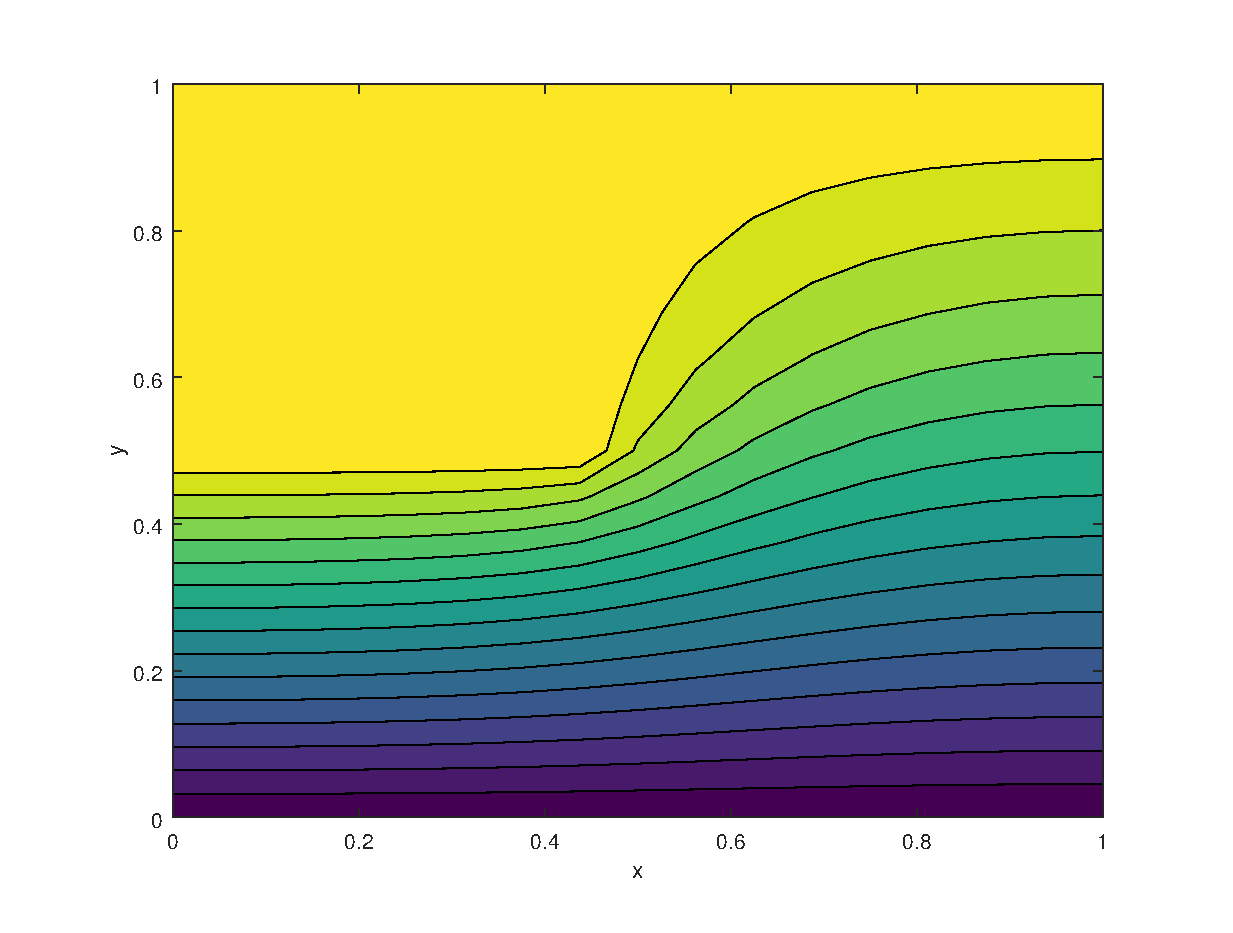
\includegraphics[scale=0.6]{eps/plotPot}
%\end{center}
%\caption[Potentialverlauf eines Kondensators mit Kante]{Potentialverlauf des Kondensators mit Kante.}
%\label{fig:V4.PA4.1}
%\end{figure}

\begin{figure}
	\centering
	\begin{tikzpicture}[scale=1]
		\begin{axis}[
		xlabel={x},
		ylabel={mode},
		%grid=major,
		cycle multi list={color list\nextlist [1 of]mark list},
		legend entries={Grundmode},
		legend style={at={(0.5,-0.2)},anchor=south},
		]
		\addplot table[x=x, y=mode1, col sep=comma] {../csv/modes.csv};
		\addplot+
%		\addplot+ [
%mark=ball,
%mark size=4pt,
%scatter,% enable scatter
%scatter src=rand,% the "color data"
%% configure individual appearances:
%scatter/use mapped color=
%{ball color=mapped color}]
coordinates
{(-0.1,0) (-1,0.1) (0,0) (0.1,0.1) (0.2,0)};

		
		
		\end{axis}
	\end{tikzpicture}
	\caption{asdf}
\end{figure}



\pgfplotstableread[col sep = comma, columns/3/.style={string type}, ignore chars= {(, ),j}] {transfer_fct.csv}\kennlinie %%%%% cannot deal with a 'j' in imaginary part! %%%
%\pgfplotstabletypeset[columns={0,3}, columns/3/.style={string type}] \kennlinie
% erzeugt eine banale Liste

\begin{figure}[hb]
\centering
    \begin{tikzpicture}
\begin{axis}[
		legend entries = {Amplitude},
		legend pos = outer north east,
		]
\addplot[blue, thick] table [ x =0, y index=1] {\kennlinie};

		\addplot [red, mark=o, mark size=5pt]coordinates {(10000000, 8)};
		\addplot coordinates{(20000000, 5)}	;	
		
\end{axis}
\end{tikzpicture}
\caption{Einzelsinus}
\end{figure}

Dies ist ein Versuch, eine Transfer-Function zu plotten mittels tikz:

%\begin{figure}[h!]
%\centering
%    \begin{tikzpicture}
%    \datavisualization [scientific axes=clean, 
%    					visualize as line, 
%    					x axis = {attribute = frequency},
%    					y axis = {attribute = amplitude}]
%    	data [read from file = transfer_fct.csv,
%    			%headline = {frequency, amplitude, phaseshift, complex}
%    			];
%    
    
%\begin{axis}[grid=both, xlabel={$t/T_{\textrm{BB}}$},
%ylabel={$\Usin(t)$},                        ytick={-1,1},
%                        yticklabels={$-\widehat{U}$,$\widehat{U}$},
%                        xtick={-4,-2,0,2,4},
%                        xticklabels={-2,-1,0,1,2}]
%\addplot[blue, thick] table [ x expr={\thisrowno{0}}, y
%expr={\thisrowno{1}}, col sep=semicolon] {csv/transfer_fct.csv};
%\end{axis}
%	\end{tikzpicture}
%\caption{Bsp-Plot einer Transfer-Function H}
%  \label{fig:bsp_transfer}
%\end{figure}


Dies ist ein Versuch, ein Frequenzspektrum zu plotten und Marker an relevanten Punkten zu setzen:




\end{document}